% Comentários % TODO: indicam tarefas não concluídas; tarefas planejadas não são resultados de teste.
% Não declarar calibração ou validação empírica como concluídas sem os dados
\documentclass[conference]{IEEEtran}

\usepackage{cite}
\usepackage{graphicx}
\usepackage{url}
\usepackage{xurl}
\usepackage{booktabs}
\usepackage{array}
\usepackage{tabularx}
\usepackage{ragged2e}
\usepackage{placeins}
\usepackage{float}
\usepackage{amsmath}
\usepackage{enumitem}
\usepackage{tikz}
\usepackage{longtable}
\usetikzlibrary{arrows.meta,positioning,shapes.geometric}

\setlist{nosep,leftmargin=*}
\renewcommand{\refname}{Referências}
\renewcommand{\tablename}{Tabela}
\renewcommand{\figurename}{Figura}
\renewcommand{\IEEEkeywordsname}{Palavras-chave}
\newcolumntype{Y}{>{\RaggedRight\arraybackslash}X}

\begin{document}

\title{Matchmaking e Cooperação em Jogos Multiplayer Online Competitivos: Modelagem do Agente Proxy UXAgent}

\author{
\IEEEauthorblockN{1\textsuperscript{st} João Pedro Rodrigues Silva}
\IEEEauthorblockA{\textit{Engenharia da Computação}\\
\textit{CEFET-MG Campus V.}\\Divinópolis, Brasil\\jprs1308@gmail.com}
\and
\IEEEauthorblockN{2\textsuperscript{nd} Pedro Augusto Gontijo Moura}
\IEEEauthorblockA{\textit{Engenharia da Computação}\\
\textit{CEFET-MG Campus V.}\\Divinópolis, Brasil\\pedroaugustomoura70927@gmail.com}
\and
\IEEEauthorblockN{3\textsuperscript{rd} Samuel Silva Gomes}
\IEEEauthorblockA{\textit{Engenharia da Computação}\\
\textit{CEFET-MG Campus V.}\\Divinópolis, Brasil\\silvagomes881@gmail.com}
}

\maketitle

\begin{abstract}
Este artigo especifica a modelagem do UXAgent, agente proxy baseado em modelo de linguagem de grande escala (LLM), para depuração de protocolos, instrumentação e métricas de Interação Humano-Computador antes de estudos com participantes. O perfil-alvo é o de adultos com experiência recente em jogos multiplayer por equipes, representado por persona fictícia e de alcance limitado. A interface pretendida é um lobby simplificado para atribuição de funções, revisão de dependências e comunicação de um plano cooperativo; o protótipo executável atual é de linha de comando e ainda não possui interface gráfica clicável. A especificação relaciona quatro manifestações funcionais a mecanismos parametrizados externos ao prompt, descreve controlador, avaliador, quatro tarefas, protocolo, eventos e métricas. Um protótipo preliminar para T1--T2 foi executado com política simulada e com a API Gemini: a suíte automatizada v2 passou em 57 testes, e os logs reais evidenciaram dois deslizes injetados de R1 recuperados em T1, repetição de pings na configuração anterior e uma execução diagnóstica posterior de T2 interrompida por falha técnica. Esses resultados verificam partes da implementação, não a validade humana do agente. Os conjuntos públicos encontrados são apenas parcialmente compatíveis com o lobby proposto; portanto, sem dados humanos compatíveis e comparação independente, o UXAgent permanece exploratório e não validado como representante de jogadores.
\end{abstract}

\begin{IEEEkeywords}
UXAgent, modelagem de usuário, jogos multiplayer, cognição distribuída, métricas de IHC, LLM.
\end{IEEEkeywords}

\section{Escopo e Delimitação do Perfil}

O UXAgent será usado para testar a consistência de instruções, critérios de sucesso, registros e cálculos de métricas em tarefas digitais controladas. Ele não implementa nem avalia causalmente algoritmos reais de matchmaking nesta etapa. O sistema experimental representa apenas um lobby e o planejamento de uma missão cooperativa fictícia; seus resultados não devem ser generalizados para partidas reais ou para todos os jogadores.

\textbf{Pergunta operacional:} como uma persona adulta com experiência em jogos multiplayer por equipes executa tarefas de atribuição de funções e planejamento cooperativo em uma interface web, e até que ponto um agente LLM parametrizado pode reproduzir padrões observáveis úteis à depuração do protocolo?

\begin{table}[!t]
\centering
\caption{Delimitação do perfil e do fenômeno de interação.}
\label{tab:tucig}
\scriptsize
\renewcommand{\arraystretch}{1.1}
\begin{tabularx}{\columnwidth}{@{}p{0.6cm}Y@{}}
\toprule
\textbf{Comp.} & \textbf{Especificação} \\
\midrule
T & Interface web controlada com lobby, cartões de integrantes, requisitos da missão, mensagens rápidas, checklist e ajuda contextual. O UXAgent seleciona ações; o controlador aplica mecanismos parametrizados e registra eventos. \\
U & Adulto (18 anos ou mais) com experiência prévia em jogos multiplayer por equipes. É uma proposta de interesse, não uma condição clínica; a persona é uma instância de projeto, não um retrato de toda a população. \\
C & Planejamento de uma missão fictícia em computador, com informações sobre integrantes e dependências de tarefas apresentadas em painéis e recursos de suporte disponíveis. \\
I & Coordenação observável na interface: atribuição válida de funções, revisão de plano após atualização, comunicação por mensagem rápida, erros, conclusão de tarefa e uso de ajuda. Cognição Distribuída orienta a análise da relação entre usuário, artefatos e informação compartilhada \cite{hollan2000}. \\
G & Hipótese operacional: um agente com mecanismos explícitos pode auxiliar a depuração de protocolos e métricas, mas a equivalência de seus padrões com os de jogadores adultos não está estabelecida. A literatura consultada não demonstra validade para esta interface e estas tarefas específicas. \\
\bottomrule
\end{tabularx}
\end{table}

O perfil foi classificado como \textit{outra proposta de interesse}, por não corresponder a uma ocupação nem a uma condição clínica. Para tornar o recorte verificável, esta versão adota como grupo-alvo adultos (18 anos ou mais) que relatem jogar partidas multiplayer por equipes pelo menos uma vez por semana nos últimos três meses. O grupo comparador será composto por adultos com familiaridade digital geral que relatem jogar esse tipo de jogo no máximo uma vez por mês nos últimos seis meses. Esses limiares são \textbf{decisões operacionais do projeto}, não resultados publicados nem definições universais de experiência; a frequência autorrelatada não será tratada como medida suficiente de habilidade. Scoggins et al. estudaram 221 adultos jogadores de 18 a 62 anos (idade média de 27,29 anos), mas não se restringiram a jogos competitivos por equipes; Nakae e Inaba analisaram proficiência e comunicação em jogo cooperativo, sem informar no artigo a faixa etária dos participantes \cite{scoggins2025,nakae2025}. As fontes justificam considerar experiência e variação individual, mas não fornecem probabilidades transferíveis para o agente. Os cortes ficam fixados nesta versão para fins de modelagem; qualquer alteração antes da coleta deverá ser datada e justificada no protocolo.

\section{Especificação da Persona}

A persona é fictícia. O nome, a idade específica e os hábitos abaixo são escolhas de projeto, não dados de uma pessoa real. A idade de 27 anos é um ponto ilustrativo próximo à idade média reportada na amostra adulta de Scoggins et al.; essa proximidade não implica representatividade para jogadores competitivos em equipe \cite{scoggins2025}.

\begin{table}[!t]
\centering
\caption{Ficha operacional da persona.}
\label{tab:persona}
\scriptsize
\renewcommand{\arraystretch}{1.12}
\begin{tabularx}{\columnwidth}{@{}p{1.45cm}Y@{}}
\toprule
\textbf{Elemento} & \textbf{Especificação e procedência} \\
\midrule
Perfil & Alex, 27 anos, adulto fictício que satisfaz o critério operacional de jogar multiplayer por equipes ao menos semanalmente nos últimos três meses. A idade é ilustrativa, próxima à média de uma amostra ampla de adultos jogadores; não implica representatividade do recorte competitivo \cite{scoggins2025}. \\
Objetivo de uso & Entender a missão, distribuir três funções complementares, ajustar o plano quando o estado da equipe muda e confirmar uma solução válida. \\
Capacidades & Reconhece elementos usuais de lobby e papéis de equipe; consegue comparar requisitos e atribuir funções; pode usar mensagens rápidas para tornar decisões compartilhadas explícitas. São competências a testar, não características universais de jogadores. \\
Experiência digital & Familiaridade com navegador, botões, cartões de informação e seleção de opções. A experiência em jogos é definida pela frequência de jogo do critério operacional; a proficiência individual não é presumida só pela frequência e deverá ser registrada separadamente no estudo futuro. \\
Contexto & Computador com mouse e teclado; missão breve, sem voz e sem movimento em tempo real. O teste usa condições iniciais controladas e eventos de estado predefinidos. \\
Recursos de suporte & Checklist de dependências, painel de estado da missão, ajuda contextual e mensagens rápidas/pings. A consulta ao checklist antes de confirmar é uma estratégia compensatória que será observada. \\
Variabilidade e limites & Jogadores diferem em proficiência, comunicação e uso de suporte. O agente não representa emoção, toxicidade, relações sociais duradouras, habilidade mecânica em partidas reais ou todos os estilos de jogo. \\
\bottomrule
\end{tabularx}
\end{table}

A persona não será instruída apenas por um parágrafo de personalidade. As diferenças de execução serão testadas por parâmetros, filtros de observação e regras de controle externos ao prompt. A amostragem e os limiares de frequência precisam ser registrados antes de qualquer coleta. Os valores iniciais apresentados a seguir servem para testar a instrumentação e não são estimativas populacionais.

Para tornar explícita a escolha de cada atributo, a faixa etária documentada na fonte consultada é de 18 a 62 anos, e Alex foi fixado em 27 anos, próximo à média de 27,29 anos da amostra de Scoggins et al. Para frequência de jogo, não foi adotada uma faixa da literatura: os cortes semanal nos últimos três meses e mensal nos últimos seis meses são critérios operacionais escolhidos pelo projeto para separar perfil e comparador. Para capacidades, familiaridade digital, contexto e uso de suporte, as fontes consultadas não fornecem uma faixa quantitativa compatível com este lobby; esses elementos são hipóteses operacionais explicitamente escolhidas para o cenário e não comportamentos obrigatórios. A variação individual e as características não representadas estão registradas na ficha, e nenhuma dessas escolhas é tratada como estimativa populacional.

% Critério operacional fixado nesta versão. Não interpretar frequência de jogo como medida isolada de habilidade nem apresentar os cortes como resultados da literatura.

\section{Fundamentação Teórica e Matriz de Rastreabilidade}

A Cognição Distribuída fundamenta a observação de como a informação é distribuída entre o jogador, o estado da missão, a interface e os demais integrantes \cite{hollan2000}. A análise hierárquica de tarefas e o GOMS dão suporte à decomposição das ações e à construção de uma linha de base operacional \cite{benyon2010,dix2004}. A ISO 9241-11 orienta a relação entre eficácia, eficiência e contexto de uso; a literatura de testes de usabilidade e de eventos da interface fundamenta o registro de sucesso, erros e sequência de ações \cite{iso9241_11,saadawi2005}. Estudos de simulação com LLMs indicam utilidade potencial para pilotagem, mas não estabelecem equivalência automática entre dados sintéticos e humanos \cite{hamalainen2023,simuser2024}. Pela classificação de Kammersgaard, a perspectiva de interação adotada é a de \textit{sistema}: o lobby é uma aplicação com comandos, regras e estados verificáveis; o UXAgent não será tratado como parceiro de diálogo para inferir relações sociais. Assim, ações são operações concretas da interface e erros são violações observáveis das regras ou do estado esperado \cite{kammersgaard1988}.

Em termos do arsenal da disciplina, objetivos de estudo, affordances e qualidade em IHC aparecem nos critérios externos de sucesso e no dicionário de métricas; psicologia cognitiva e engenharia cognitiva aparecem nos mecanismos de observação desatualizada, decisão e ação; Cognição Distribuída aparece na relação entre feed, cartões e plano; análise de tarefas e GOMS aparecem na HTA e na linha de base de ações; e avaliação de interfaces aparece no protocolo, nas categorias de erro, nos eventos e na análise de incerteza. Os subsídios específicos de jogos e de LLMs complementam esses modelos, mas não os substituem.

\begin{table*}[!t]
\centering
\caption{Matriz de rastreabilidade: característica, mecanismo e previsão.}
\label{tab:matriz}
\scriptsize
\renewcommand{\arraystretch}{1.12}
\setlength{\tabcolsep}{3pt}
\begin{tabularx}{\textwidth}{@{}>{\RaggedRight\arraybackslash}p{1.9cm}>{\RaggedRight\arraybackslash}p{2.45cm}>{\RaggedRight\arraybackslash}p{1.9cm}>{\RaggedRight\arraybackslash}p{2.85cm}>{\RaggedRight\arraybackslash}p{2.9cm}Y@{}}
\toprule
\textbf{Característica e fonte} & \textbf{Manifestação e demanda da interface} & \textbf{Modelo/método IHC} & \textbf{Mecanismo e parâmetro candidato} & \textbf{Evento, métrica e previsão} & \textbf{Pressupostos, limitações e situação} \\
\midrule
\textbf{R1 -- Variação da execução válida}\\Nakae e Inaba, §§3.1--3.3, pp. 766--767; Zhang et al., resumo e §§3.2, 4.2--4.4, pp. 3644--3653 \cite{nakae2025,quickskill2022}. &
Selecionar funções válidas e respeitar os requisitos apresentados nos cartões da equipe e da missão. &
Análise de tarefas; GOMS; eficácia de usabilidade. &
$p_{\mathrm{valida}}=0{,}90$, faixa de sensibilidade $[0{,}60;0{,}95]$. Em cada oportunidade predefinida, o controlador mantém a ação candidata com essa probabilidade; caso injete um deslize, seleciona uma alternativa permitida pela interface, mas incompatível com uma regra do plano. Se não houver alternativa errada legal, a injeção não ocorre. &
Registrar ação proposta/executada, atribuição incompatível, erro e estado final. Reduzir o parâmetro deve aumentar os erros injetados e reduzir o sucesso no mesmo cenário controlado. &
A literatura sustenta a relevância da proficiência, mas não estima esta probabilidade. Valor e faixa são hipóteses operacionais para depuração, não uma estimativa sobre jogadores. Estado: hipótese operacional. \\
\midrule
\textbf{R2 -- Coordenação explícita}\\Nakae e Inaba, §4 e análise de comunicação, pp. 768--771; Cole e Griffiths, método/participantes, p. 576, e conclusão, p. 582 \cite{nakae2025,cole2007}. &
Atribuições e mudanças de plano podem exigir que a decisão seja comunicada a outros integrantes por ping/mensagem rápida. &
Cognição Distribuída; análise de tarefas; interação social. &
\texttt{p\_comunicar = 0,65}, faixa [0,20; 0,90]. Em uma oportunidade de comunicação, o controlador habilita a ação de mensagem conforme o parâmetro. A mensagem é uma ação explícita, nunca inferida do texto interno do LLM. &
Registrar tipo e momento do ping, ação antes/depois da mensagem e envio de plano sem aviso. Aumentar o parâmetro deve elevar a frequência de eventos de comunicação; efeito sobre sucesso não é presumido. &
Há evidência de diálogo e colaboração em tarefa distinta; os valores numéricos são provisórios e a transferência para um lobby competitivo é inferência. Estado: hipótese operacional. \\
\midrule
\textbf{R3 -- Replanejamento diante de mudança}\\Nakae e Inaba, §§3.1--3.2, pp. 766--767; Hollan et al., artigo conceitual, pp. 174--196 \cite{nakae2025,hollan2000}. &
Uma atualização do estado do integrante pode invalidar uma atribuição anterior e exigir revisão do plano. &
Cognição Distribuída; análise de tarefas; avaliação por eventos. &
\texttt{p\_estado\_fresco = 0,70}, faixa [0,30; 0,95]. Quando uma atualização torna o plano inconsistente, o controlador expõe o estado atualizado ao agente com a probabilidade definida; caso contrário, mantém a observação anterior em cache para testar o efeito de informação desatualizada. &
Registrar atualização, revisão, tentativa de confirmação com estado obsoleto e erros de dependência. Aumentar o parâmetro deve reduzir submissões de planos obsoletos no mesmo cenário. &
A atualização é mecanismo de teste controlado; não prova um processo cognitivo humano. O valor não é estimado nas fontes. Estado: hipótese operacional. \\
\midrule
\textbf{R4 -- Estratégia compensatória de suporte}\\ISO 9241-11:2018, conceitos de eficácia/eficiência; NIST, página institucional sobre testes de usabilidade; Saadawi et al., método/avaliação, pp. 654--658 \cite{iso9241_11,nistUsability,saadawi2005}. &
Quando há dependência não resolvida, a persona pode consultar o checklist de base; a ajuda contextual oferece uma segunda fonte de suporte antes de confirmar. &
Eficácia/eficiência; suporte à tarefa; registro de eventos. &
\texttt{p\_ajuda\_exposta = 0,25}, faixa [0,00; 0,80]. Em uma oportunidade de incerteza predefinida, o controlador inclui a ação \texttt{open\_help(topic)} na observação com essa probabilidade; o checklist permanece disponível como suporte de base. Se acionada, a ajuda contextual revela a pré-condição faltante. O LLM ainda decide se executa a ação, e a métrica registra somente o uso efetivo. O parâmetro controla a disponibilidade da affordance, não uma probabilidade humana de buscar ajuda. &
Registrar abertura de ajuda, condição que a disparou, ações posteriores e erro/sucesso. O parâmetro prevê frequência de suporte; o efeito na correção é medido, não pressuposto como fato humano. &
Inclui uma estratégia de apoio e uma capacidade preservada, não apenas uma dificuldade. A probabilidade é uma hipótese de projeto. Estado: hipótese operacional. \\
\bottomrule
\end{tabularx}
\end{table*}

Os parâmetros numéricos da Tabela~\ref{tab:matriz} são valores iniciais de engenharia para testar o controlador, os logs e a sensibilidade das métricas. Nenhuma fonte fornece estimativas diretamente transferíveis para essas probabilidades no lobby proposto. Por isso, são valores de injeção/controle, não uma distribuição real de comportamento humano. O rótulo “proficiência” não deve ser inferido de $p_{\mathrm{valida}}$: o parâmetro manipula deliberadamente a validade de ações para testar o instrumento. Cada linha será exercitada ao menos por uma tarefa de calibração e uma tarefa reservada para validação (Seção~\ref{sec:tarefas}).

% Rastreabilidade bibliográfica: as localizações acima foram conferidas nas versões publicadas disponíveis. Para a norma ISO e a página NIST, a localização é conceitual/institucional, não uma página paginada; não atribuir-lhes paginação não verificada. Se a versão local de algum PDF divergir, atualizar a localização antes da entrega.

\section{Arquitetura do Agente}

A arquitetura separa ambiente, observação, estado e parâmetros da persona, política do LLM, controlador de ações, instrumentação e avaliador externo. O LLM recebe somente o estado que a interface disponibiliza após a transformação parametrizada e retorna uma ação estruturada escolhida entre as ações permitidas. O controlador aplica os mecanismos R1--R4 fora do prompt, verifica pré-condições, executa ou rejeita ações e atualiza o ambiente. A instrumentação registra propostas e ações realmente executadas. Um avaliador externo calcula sucesso e erros a partir do estado da interface; seus critérios e resultados não são fornecidos ao LLM.

\begin{figure*}[!t]
\centering
\resizebox{\textwidth}{!}{%
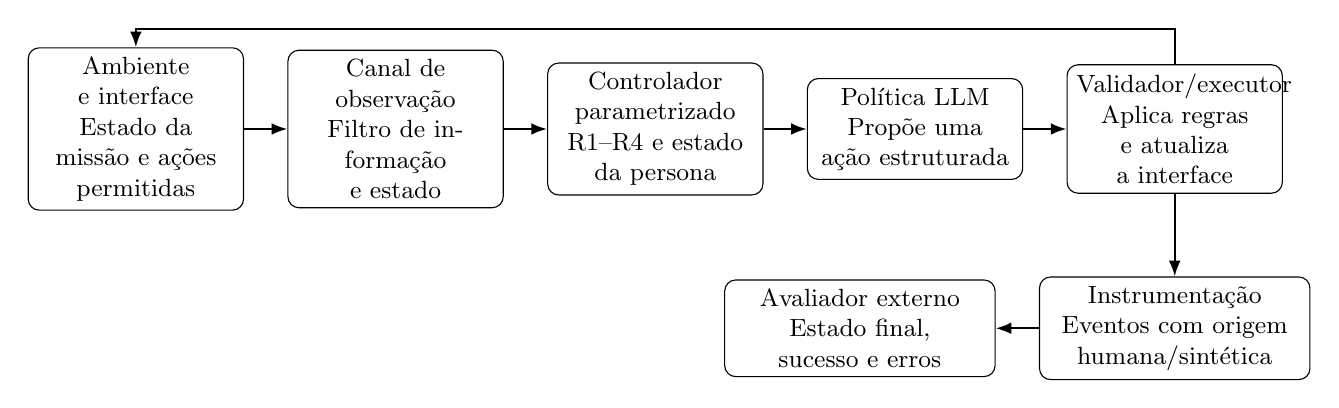
\begin{tikzpicture}[
  node distance=0.55cm,
  block/.style={draw,rounded corners,align=center,minimum height=1.15cm,text width=2.5cm,font=\small},
  aux/.style={draw,rounded corners,align=center,minimum height=0.9cm,text width=3.2cm,font=\small},
  arrow/.style={-{Latex[length=2mm]},thick}
]
\node[block] (ui) {Ambiente e interface\\Estado da missão e ações permitidas};
\node[block,right=of ui] (obs) {Canal de observação\\Filtro de informação e estado};
\node[block,right=of obs] (ctrl) {Controlador parametrizado\\R1--R4 e estado da persona};
\node[block,right=of ctrl] (llm) {Política LLM\\Propõe uma ação estruturada};
\node[block,right=of llm] (valid) {Validador/executor\\Aplica regras e atualiza a interface};
\draw[arrow] (ui) -- (obs);
\draw[arrow] (obs) -- (ctrl);
\draw[arrow] (ctrl) -- (llm);
\draw[arrow] (llm) -- (valid);
\draw[arrow] (valid.north) -- ++(0,0.45) -| (ui.north);
\node[aux,below=1.05cm of valid] (log) {Instrumentação\\Eventos com origem humana/sintética};
\node[aux,left=0.55cm of log] (eval) {Avaliador externo\\Estado final, sucesso e erros};
\draw[arrow] (valid.south) -- (log.north);
\draw[arrow] (log.west) -- (eval.east);
\end{tikzpicture}%
}
\caption{Arquitetura proposta do UXAgent. O avaliador e os logs não expõem o gabarito ao LLM.}
\label{fig:arquitetura}
\end{figure*}

\subsection{Componentes e regras}
\begin{itemize}
\item \textbf{Ambiente/interface:} apresenta cartões de integrantes, requisitos, dependências, mensagens rápidas, checklist e botão de confirmação. Mantém o estado verdadeiro da missão.
\item \textbf{Canal de observação:} converte o estado em uma observação serializada e aplica a condição de visibilidade/informação desatualizada definida por R3.
\item \textbf{Estado e configuração da persona:} armazena perfil fictício, tarefa corrente, estado observado e parâmetros. Os valores são externos ao prompt, versionados e passíveis de desligamento.
\item \textbf{Política LLM:} escolhe a próxima ação dentre um conjunto enumerado, sem receber o gabarito nem a função de avaliação.
\item \textbf{Controlador/validador:} executa R1--R4, impede ações fora do vocabulário permitido, classifica falhas e atualiza o estado; as chaves de cada mecanismo permitem comparação em condição neutra.
\item \textbf{Instrumentação/avaliador:} gera logs auditáveis e determina resultados a partir do estado da aplicação, sem depender da declaração do agente.
\end{itemize}

A configuração neutra desliga R1--R4 e deixa a política do mesmo LLM escolher ações legalmente disponíveis; ela é um controle técnico, não um controle humano. Para testar se R1 afeta os indicadores, propõe-se comparar provisoriamente $p_{\mathrm{valida}}=0{,}90$ e $p_{\mathrm{valida}}=0{,}60$, mantendo R2--R4 fixos. Isso isola a injeção de deslizes e não representa, por si só, jogadores experientes e novatos. Um executor determinístico baseado em regras será usado como controle de sanidade para testar critérios de sucesso, logs e fórmulas; seus resultados não serão tratados como dados humanos. A sensibilidade será testada variando um parâmetro por vez dentro das faixas declaradas e, quando viável, verificando combinações de mecanismos.

O LLM deverá retornar uma ação estruturada a partir do vocabulário fechado definido no arquivo auxiliar \texttt{uxagent\_action.schema.json}: \texttt{select\_role(member, role)}, \texttt{set\_step\_order(steps)}, \texttt{send\_ping(code)}, \texttt{open\_checklist()}, \texttt{open\_help(topic)}, \texttt{refresh\_feed()}, \texttt{review\_plan()} e \texttt{confirm\_plan()}. \texttt{set\_step\_order} escolhe uma permutação das três etapas; o controlador verifica dependências e pode rejeitar ordens incompatíveis. \texttt{open\_checklist} é distinto de \texttt{open\_help}, para que o uso de cada recurso possa ser registrado separadamente. A saída deverá obedecer a um esquema estruturado (JSON Schema), rejeitando campos desconhecidos, nomes de ação fora do vocabulário ou argumentos incompatíveis com a tarefa. O controlador valida tipo, argumentos e pré-condições antes da execução. Registrar todos os parâmetros de geração documentados e usar semente apenas se a API a oferecer; não pressupor que o endpoint aceite temperatura ou semente. A saída estruturada restringe o formato, mas não garante que o modelo escolha sempre a mesma ação. A política será isolada por um adaptador de modelo, sem acoplar o restante do controlador ao fornecedor.

Como candidato inicial para a implementação, esta versão adota provisoriamente a Gemini API com o identificador de modelo \texttt{gemini-3.5-flash-lite}, usando o SDK oficial \texttt{google-genai} e saída estruturada em JSON Schema. A documentação do Google lista esse identificador como estável, orientado a tarefas agentivas de alto volume, e inclui suporte a saída estruturada; a tabela de preços consultada em 16/10/2026 mostra uso sem custo financeiro no nível gratuito \cite{gemini_model,gemini_structured,gemini_pricing}. Essa disponibilidade, os limites de chamadas e os termos podem mudar e devem ser confirmados no Google AI Studio antes da execução. A tabela oficial também indica que o conteúdo do nível gratuito pode ser usado para melhorar produtos do Google. Portanto, essa modalidade será usada somente com cenários sintéticos/fictícios; não serão enviados dados, registros, transcrições ou identificadores de participantes humanos. A API pode aceitar apenas um subconjunto de JSON Schema; por isso, o controlador deverá validar a resposta integralmente com o schema local e rejeitar ações/argumentos inválidos. A seleção é provisória e não resulta de benchmark do projeto. O adaptador manterá o restante do controlador independente do fornecedor. Para reprodutibilidade, registrar modelo retornado, data, SDK/versão, versão do prompt/schema e parâmetros efetivamente suportados; não pressupor controle de semente ou determinismo se o endpoint não os oferecer.

\section{Interface, Tarefas e Análise de Tarefas}
\label{sec:tarefas}

A interface de baixa fidelidade contém: (i) painel da missão com objetivo e pré-condições; (ii) cartões dos integrantes com disponibilidade e competência relevante; (iii) seletores de função; (iv) feed de estado da equipe; (v) mensagens rápidas/pings; (vi) checklist/ajuda contextual; e (vii) resumo do plano e botão \textit{Confirmar}. As três funções da missão são localizar o recurso, ativar o ponto de controle e transportar o recurso à extração. O plano só é válido se todas as funções estiverem atribuídas uma única vez a integrantes disponíveis e as dependências forem respeitadas: o transporte só pode ser concluído depois da localização do recurso e da ativação do ponto de controle. O estado final será verificado por uma regra externa.

\begin{table}[!t]
\centering
\caption{Telas, elementos e ações permitidas na interface de teste.}
\label{tab:interface}
\scriptsize
\renewcommand{\arraystretch}{1.08}
\begin{tabularx}{\columnwidth}{@{}p{1.45cm}Y Y@{}}
\toprule
\textbf{Área/tela} & \textbf{Elementos observáveis} & \textbf{Ações permitidas}
\\
\midrule
Missão & Objetivo, três funções, dependências e regra de confirmação. & Consultar requisitos; \texttt{open\_checklist()} ou \texttt{open\_help(topic)}. \\
Equipe & Cartões com identificador fictício, disponibilidade e capacidade para cada função. & \texttt{select\_role(member, role)} para atribuir ou alterar função; consultar cartão. \\
Feed da equipe & Atualizações de estado e aviso de indisponibilidade. & \texttt{refresh\_feed()} e \texttt{send\_ping(code)}; ler nova condição. \\
Plano & Resumo das funções e sequência proposta. & \texttt{set\_step\_order(steps)}, \texttt{review\_plan()} e \texttt{confirm\_plan()}. \\
\bottomrule
\end{tabularx}
\end{table}

\begin{figure*}[!t]
\centering
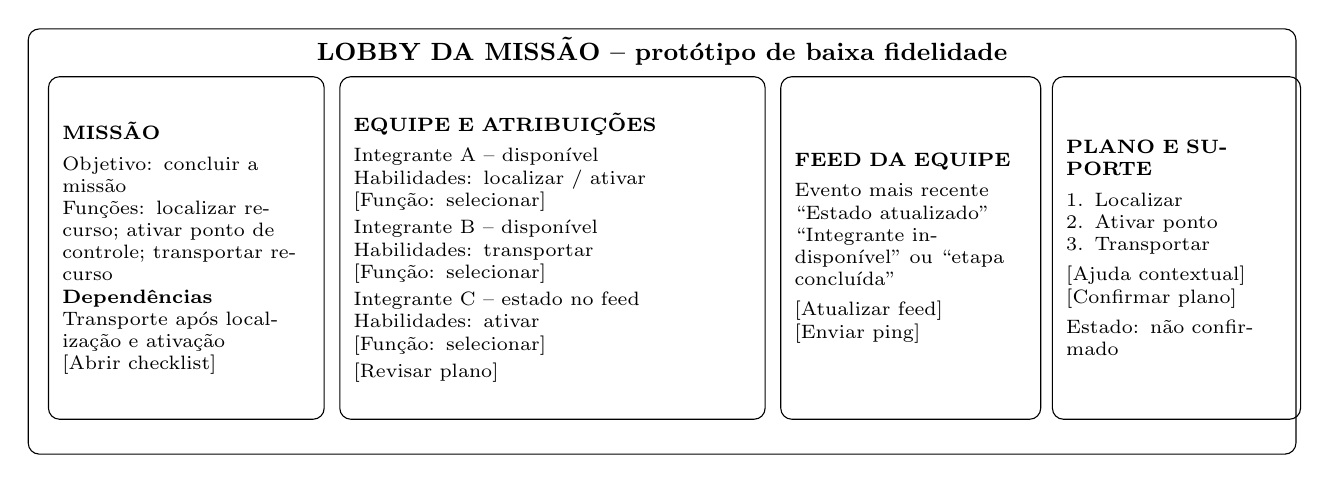
\begin{tikzpicture}[
  font=\scriptsize,
  panel/.style={draw,rounded corners,align=left,anchor=north west,inner sep=5pt,minimum height=4.35cm},
  heading/.style={font=\bfseries\small}
]
  \draw[rounded corners] (0,0) rectangle (16.1,5.4);
  \node[heading] at (8.05,5.12) {LOBBY DA MISSÃO -- protótipo de baixa fidelidade};
  \node[panel,text width=3.15cm,minimum width=3.45cm] (mission) at (0.25,4.8) {\textbf{MISSÃO}\\[3pt]
    Objetivo: concluir a missão\par
    Funções: localizar recurso; ativar ponto de controle; transportar recurso\par
    \textbf{Dependências}\par
    Transporte após localização e ativação\par
    [Abrir checklist]};
  \node[panel,text width=5.05cm,minimum width=5.35cm] (team) at (3.95,4.8) {\textbf{EQUIPE E ATRIBUIÇÕES}\\[3pt]
    Integrante A -- disponível\par
    Habilidades: localizar / ativar\par
    [Função: selecionar]\par\vspace{2pt}
    Integrante B -- disponível\par
    Habilidades: transportar\par
    [Função: selecionar]\par\vspace{2pt}
    Integrante C -- estado no feed\par
    Habilidades: ativar\par
    [Função: selecionar]\par\vspace{2pt}
    [Revisar plano]};
  \node[panel,text width=2.95cm,minimum width=3.25cm] (feed) at (9.55,4.8) {\textbf{FEED DA EQUIPE}\\[3pt]
    Evento mais recente\par
    ``Estado atualizado''\par
    ``Integrante indisponível'' ou ``etapa concluída''\par\vspace{3pt}
    [Atualizar feed]\par
    [Enviar ping]};
  \node[panel,text width=2.8cm,minimum width=3.05cm] (plan) at (13.0,4.8) {\textbf{PLANO E SUPORTE}\\[3pt]
    1. Localizar\par
    2. Ativar ponto\par
    3. Transportar\par\vspace{3pt}
    [Ajuda contextual]\par
    [Confirmar plano]\par\vspace{3pt}
    Estado: não confirmado};
\end{tikzpicture}
\caption{Wireframe da interface proposta. Os cartões de integrantes são ilustrativos e se repetem conforme a tarefa; a implementação deverá manter este vocabulário de ações ou atualizar protocolo, tarefas e esquema de eventos em conjunto.}
\label{fig:wireframe}
\end{figure*}

% O wireframe atende à representação preliminar exigida na modelagem; ainda não é uma captura de protótipo funcional.

As tarefas T1--T2 são de calibração. T3--T4 ficam reservadas para validação independente. A especificação detalhada dos cenários, estados iniciais e critérios externos está registrada separadamente em \texttt{Tarefas\_validacao\_reservadas\_v1.md}, versão 1.0, congelada em 20/10/2026. O SHA-256 do arquivo é apresentado em quatro blocos para evitar quebra automática do identificador:
\begin{center}
\small
\textit{SHA-256 do artefato}\par
\texttt{64e658adbe4c16a5e0bf5c630947c308}\par
\texttt{9e0f432f94fb794a0522a7c327b64649}
\end{center}
O arquivo reservado não deve ser incluído no prompt, na memória recuperada, nos exemplos ou nos dados de calibração do LLM. Se for alterado depois de consultar qualquer resultado de T3/T4, esta versão deixa de ser uma validação independente e um novo conjunto de tarefas deverá ser reservado.

\subsection{T1 -- Atribuir as funções no lobby (calibração)}
\textbf{Objetivo:} atribuir as três funções complementares aos três integrantes disponíveis sem duplicação. \textbf{Pré-condições:} missão nova, nenhum papel atribuído e todos os cartões visíveis. \textbf{Entradas:} três cartões com disponibilidade/competências, as três funções e suas dependências; plano inicialmente vazio. \textbf{Procedimento/HTA:} 1) ler requisitos; 2) consultar cartões; 3) atribuir cada função com \texttt{select\_role} (três vezes); 4) acionar \texttt{review\_plan}; 5) acionar \texttt{confirm\_plan}. \textbf{Sucesso verificável:} três funções atribuídas exatamente uma vez, nenhum integrante indisponível e plano confirmado em estado válido. \textbf{Erros possíveis:} função omitida/duplicada, atribuição a integrante indisponível, confirmação prematura ou ação rejeitada. \textbf{Cobertura:} R1. \textbf{Cenário:} Alex entra em um lobby recém-criado e precisa organizar a equipe antes da missão. \textbf{Dificuldade:} baixa a moderada; há três associações sujeitas a unicidade e compatibilidade, leitura curta de dois tipos de informação (requisitos e cartões) e uma verificação final; não há atualização de estado durante a tarefa.

\textbf{Relação HTA:} ler requisitos $\rightarrow$ consultar cartões $\rightarrow$ atribuir as três funções (repetir três vezes) $\rightarrow$ revisar o plano $\rightarrow$ confirmar. A ordem é obrigatória. Oportunidades de erro: cada atribuição e a confirmação final.

\textbf{GOMS de referência:} \texttt{M M (P K)$^3$ M P K M P K}. Contagem prevista: 4 operadores mentais (M), 5 apontamentos (P) e 5 ativações (K), total de 14 operadores; são cinco ações de interface observáveis (três atribuições, revisão e confirmação). A contagem não é tempo humano.

\subsection{T2 -- Revisar plano após atualização e comunicar a equipe (calibração)}
\textbf{Objetivo:} ajustar a sequência do plano após uma atualização de estado e comunicar a mudança antes de confirmar. \textbf{Pré-condições:} há uma atribuição inicial válida; o estado da equipe muda durante a tarefa e o feed contém uma atualização relevante. \textbf{Entradas:} plano inicial, dependências da missão e aviso de atualização no feed. \textbf{Procedimento/HTA:} 1) ler missão e plano inicial; 2) acionar \texttt{refresh\_feed()} e conferir o estado novo; 3) definir a sequência com \texttt{set\_step\_order(steps)}; 4) enviar \texttt{send\_ping(PLAN\_UPDATED)}; 5) consultar \texttt{open\_checklist()} quando necessário ou \texttt{open\_help(topic)} se a ajuda contextual estiver exposta por R4; 6) acionar \texttt{review\_plan()} e depois \texttt{confirm\_plan()}. \textbf{Sucesso verificável:} sequência compatível com o estado atualizado, ping enviado e confirmação válida. O suporte é opcional e seu uso é medido, não obrigatório. \textbf{Erros possíveis:} usar estado antigo, ignorar dependência, não comunicar a mudança ou confirmar plano inválido. \textbf{Cobertura:} R2, R3 e R4. \textbf{Cenário:} o lobby atualiza a situação do recurso depois que Alex começou a organizar a missão. \textbf{Dificuldade:} moderada; exige atualizar e reler o feed, reinterpretar as dependências, ordenar três etapas, comunicar a mudança e rever o resultado; a ajuda introduz um caminho alternativo.

\textbf{Relação HTA:} ler missão/plano $\rightarrow$ atualizar feed $\rightarrow$ integrar a informação nova $\rightarrow$ definir a sequência $\rightarrow$ enviar ping $\rightarrow$ consultar suporte opcionalmente $\rightarrow$ revisar plano $\rightarrow$ confirmar. Oportunidades: atualizar a observação, respeitar a dependência, comunicar a mudança e confirmar apenas plano válido.

\textbf{GOMS de referência:} \texttt{M M P K M P K M P K [P K] P K M P K}. Sem suporte: 5 operadores mentais (M), 5 apontamentos (P) e 5 ativações (K), total de 15 operadores; com uma consulta de suporte: 5 M, 6 P e 6 K, total de 17. A referência corresponde a cinco ações obrigatórias, mais uma ação opcional de suporte.

\subsection{T3 -- Replanejar após indisponibilidade de integrante (validação reservada)}
\textbf{Objetivo:} corrigir uma atribuição existente após um integrante tornar-se indisponível. \textbf{Pré-condições:} plano parcialmente preenchido; após a observação inicial, um integrante atribuído fica indisponível; existe distribuição alternativa válida. \textbf{Entradas:} plano parcial, três funções, cartões dos integrantes e atualização de indisponibilidade no feed. \textbf{Procedimento/HTA:} 1) ler o plano e os cartões iniciais; 2) acionar \texttt{refresh\_feed()} e verificar o estado atualizado; 3) identificar a atribuição invalidada; 4) redistribuir as três funções usando \texttt{select\_role} (três vezes); 5) acionar \texttt{review\_plan()}; 6) confirmar com \texttt{confirm\_plan()}. \textbf{Sucesso verificável:} nenhuma função fica atribuída ao integrante indisponível, todas as funções são cobertas e o plano satisfaz as dependências. \textbf{Erros possíveis:} não atualizar o feed, manter a atribuição invalidada, duplicar função, deixar função sem responsável ou confirmar sem revisar. \textbf{Cobertura:} R1 e R3. \textbf{Cenário:} pouco antes da confirmação, um membro sai da equipe e Alex deve recuperar o plano. A combinação concreta de integrantes e restrições não será usada na calibração. \textbf{Dificuldade:} moderada a alta; é necessário detectar uma mudança posterior à observação inicial e reparar uma distribuição parcial, preservando disponibilidade, unicidade e dependências ao mesmo tempo.

\textbf{Relação HTA:} ler plano/cartões $\rightarrow$ atualizar feed $\rightarrow$ localizar atribuição inválida $\rightarrow$ escolher substitutos $\rightarrow$ verificar cobertura/dependências $\rightarrow$ revisar $\rightarrow$ confirmar. Oportunidades: atualizar a observação, retirar a atribuição inválida, cobrir todas as funções e não confirmar com dependência violada.

\textbf{GOMS de referência:} \texttt{M M P K M (P K)$^3$ M P K M P K}. Contagem prevista: 5 operadores mentais (M), 6 apontamentos (P) e 6 ativações (K), total de 17 operadores (atualizar feed, três atribuições, revisão e confirmação). Operadores mentais não entram nos logs.

\subsection{T4 -- Integrar informações de painéis distintos (validação reservada)}
\textbf{Objetivo:} integrar o estado da missão e o feed da equipe, identificar uma dependência ainda não satisfeita, comunicar o próximo passo e confirmar um plano válido. \textbf{Pré-condições:} o requisito relevante está distribuído entre o painel da missão e o feed; uma atualização ocorre após a primeira leitura. \textbf{Entradas:} requisitos/dependências no painel da missão, estado parcial do plano e aviso novo no feed. \textbf{Procedimento/HTA:} 1) ler o painel da missão; 2) acionar \texttt{refresh\_feed()} e identificar a atualização; 3) integrar os requisitos dos dois painéis; 4) definir a sequência com \texttt{set\_step\_order(steps)}; 5) consultar \texttt{open\_checklist()} quando necessário ou \texttt{open\_help(topic)} se a ajuda contextual estiver exposta por R4; 6) enviar \texttt{send\_ping(NEXT\_STEP\_ACTIVATE\_CHECKPOINT)}; 7) acionar \texttt{review\_plan()} e \texttt{confirm\_plan()}. \textbf{Sucesso verificável:} plano compatível com ambos os painéis, dependência respeitada, ping enviado e confirmação válida. \textbf{Erros possíveis:} ignorar atualização, não consultar a fonte necessária, omitir dependência ou confirmar estado incompatível. \textbf{Cobertura:} R2, R3 e R4. \textbf{Cenário:} Alex precisa combinar a informação da missão com a atividade registrada pelos colegas; a dependência e a distribuição de informação são diferentes das de T2. \textbf{Dificuldade:} alta em relação às outras tarefas; a informação está distribuída em dois painéis, uma atualização chega depois da primeira leitura, e o plano exige integrar regras, reordenar etapas, comunicar a decisão e confirmar só após rechecagem. O suporte é uma rota alternativa.

\textbf{Relação HTA:} ler missão $\rightarrow$ atualizar feed $\rightarrow$ integrar atualização e dependência $\rightarrow$ definir sequência $\rightarrow$ consultar suporte opcionalmente $\rightarrow$ enviar ping $\rightarrow$ revisar plano $\rightarrow$ confirmar. Oportunidades: consultar o feed atualizado, integrar a dependência, comunicar a mudança e não confirmar estado incompatível.

\textbf{GOMS de referência:} \texttt{M P K M P K M [P K] P K M P K M P K}. Contagem sem suporte: 5 operadores mentais (M), 5 apontamentos (P) e 5 ativações (K), total de 15 operadores; com uma consulta de suporte: 5 M, 6 P e 6 K, total de 17. A tarefa exige integrar fontes distintas antes de decidir, em vez de apenas reparar uma atribuição.

\begin{table}[!t]
\centering
\caption{Cobertura das linhas de rastreabilidade pelas tarefas.}
\label{tab:cobertura}
\scriptsize
\begin{tabularx}{\columnwidth}{@{}p{0.65cm}Y c c@{}}
\toprule
\textbf{Linha} & \textbf{Manifestação} & \textbf{Calibração} & \textbf{Validação} \\
\midrule
R1 & Seleção de ação/atribuição válida & T1 & T3 \\
R2 & Comunicação explícita & T2 & T4 \\
R3 & Atualização/replanejamento & T2 & T4 \\
R4 & Consulta à ajuda/checklist como estratégia de suporte & T2 & T4 \\
\bottomrule
\end{tabularx}
\end{table}

Nos esquemas GOMS, M representa preparação mental estimada para a tarefa, P representa apontar para um controle e K representa ativar/clicar nesse controle. M não é registrado como evento. Como a instrumentação desta interface não mede trajetória do cursor, a linha de base comparável será formada pelas ações/ativações executadas e pela sua ordem, não pela soma total de operadores. Não haverá conversão para segundos. O vocabulário executável abrange atribuição (\texttt{select\_role}), definição da sequência (\texttt{set\_step\_order}), atualização do feed, ping, checklist, ajuda, revisão e confirmação. Textos livres e comunicação por voz ficam fora do escopo. As contagens de referência são estimativas do método especificado e deverão ser auditadas quando os controles clicáveis forem implementados.

% TODO: Depois que a interface clicável for implementada, auditar as contagens GOMS contra as ações reais. Se uma operação exigir mais de um clique ou o fluxo diferir do wireframe, atualizar operadores, tarefas, eventos e testes.

\section{Protocolo Experimental}

Será usado um protocolo comum para condições humanas e sintéticas. Qualquer diferença inevitável entre a execução de um LLM e a de uma pessoa será registrada. O protocolo apresentado descreve o plano para etapas futuras; nenhuma coleta com participantes é realizada por este documento.

\begin{table}[!t]
\centering
\caption{Protocolo comum de execução.}
\label{tab:protocolo}
\scriptsize
\renewcommand{\arraystretch}{1.08}
\begin{tabularx}{\columnwidth}{@{}p{1.35cm}Y@{}}
\toprule
\textbf{Item} & \textbf{Regra operacional} \\
\midrule
Instrução & ``Organize as funções da equipe e confirme um plano que atenda aos requisitos da missão. Use os recursos de comunicação e suporte disponíveis quando considerar necessário. A tarefa termina ao confirmar um plano ou atingir o limite de ações.'' \\
Estado inicial & Carregar a configuração predefinida da tarefa, zerar o histórico da sessão e inicializar os cartões/estado indicado na especificação da tarefa. \\
Sucesso & O avaliador externo verifica cobertura de funções, disponibilidade dos integrantes, dependências e estado de confirmação. O LLM não determina o próprio sucesso. \\
Erros & Registrar ação inválida, violação de requisito, violação de sequência/dependência, uso de estado obsoleto e omissão em oportunidade definida. A classificação é operacional; não infere estado mental não observável. \\
Interrupção & Limite inicial de 30 ações executadas por tarefa ou encerramento explícito. Sessão incompleta com log íntegro conta como não sucesso; perda técnica de log é reportada separadamente. \\
Ajuda & Checklist e ajuda contextual disponíveis nas quatro tarefas. Cada abertura e o painel exibido são registrados. \\
Eventos & Ações propostas e executadas, mudança de estado, atribuições, mensagens, suporte, confirmação, erro e falha técnica. Todos os registros do agente recebem marca sintética. \\
Comparador & Futuro grupo de adultos (18+) com familiaridade digital geral e frequência de jogo em equipe de no máximo uma vez por mês nos últimos seis meses; comparar com adultos que joguem pelo menos semanalmente nos últimos três meses. Controlar dispositivo, instruções, ajuda e ordem. Os limiares são operacionais e devem ser confirmados antes de recrutamento. \\
\bottomrule
\end{tabularx}
\end{table}

A ordem das tarefas será fixa nas verificações técnicas iniciais. Na avaliação humana formal, a ordem deverá ser contrabalanceada ou aleatorizada, mantendo as condições de interface e instrução constantes. T3 e T4 permanecerão reservadas, sem ajuste de parâmetros, exemplos ou seleção de regras com base em seus resultados. Alterações após abertura da validação exigem novo conjunto independente de tarefas. Falhas técnicas serão reportadas separadamente dos erros funcionais; intenção ou estado mental não será inferido somente do texto produzido pelo LLM.

\section{Instrumentação e Dicionário de Métricas}

Cada interação será registrada como evento estruturado. O esquema mínimo deverá permitir reconstruir a sequência, distinguir proposta do LLM de execução real, reproduzir o estado da interface e identificar a origem sintética.

\begin{table}[!t]
\centering
\caption{Esquema mínimo de eventos registrados.}
\label{tab:eventos}
\scriptsize
\renewcommand{\arraystretch}{1.08}
\begin{tabularx}{\columnwidth}{@{}p{1.55cm}Y@{}}
\toprule
\textbf{Chaves do log} & \textbf{Finalidade} \\
\midrule
\shortstack[l]{\texttt{sid}\\\texttt{tid}\\\texttt{cond}} & Identificar sessão, tarefa e condição experimental. \\
\shortstack[l]{\texttt{actor}\\\texttt{synthetic}\\\texttt{cfg\_ver}} & Identificar executor, origem humana/sintética e versão da configuração. \\
\shortstack[l]{\texttt{step}\\\texttt{event}\\\texttt{ts\_sys}} & Reconstruir a ordem dos eventos; o horário do sistema não é tempo comportamental. \\
\shortstack[l]{\texttt{obs\_id}\\\texttt{state\_pre}\\\texttt{state\_post}} & Relacionar a observação dada ao agente à mudança real do estado da interface. \\
\shortstack[l]{\texttt{act\_prop}\\\texttt{act\_exec}\\\texttt{reject}} & Diferenciar proposta do LLM, ação executada e motivo de rejeição pelo controlador. \\
\shortstack[l]{\texttt{support}\\\texttt{error}\\\texttt{opp\_id}} & Registrar suporte, categoria de erro e oportunidade predefinida. \\
\shortstack[l]{\texttt{outcome}\\\texttt{tech\_fail}} & Registrar o resultado do avaliador externo e separar falha técnica de insucesso funcional. \\
\bottomrule
\end{tabularx}
\end{table}

A Tabela~\ref{tab:eventos} define as chaves abreviadas do esquema de log; não representa dados coletados. Os eventos mínimos cobrem: início e fim da tarefa; emissão de observação; proposta, rejeição e execução de ação; mudança de estado; abertura de suporte; registro de erro; envio do plano; avaliação externa; e falha técnica. Para cada sessão serão guardados os parâmetros ativos, as versões da interface, do modelo e do controlador, o identificador da configuração e o resultado externo. O campo \texttt{synthetic} identifica a origem da sessão/dado: sessões do agente usam \texttt{true} e sessões humanas usam \texttt{false}, com identificadores pseudonimizados quando aplicável. O vocabulário e os tipos de campos foram formalizados no artefato \texttt{uxagent\_event.schema.json} (JSON Schema Draft 2020-12). O artefato é o contrato de validação do log; qualquer alteração nele deverá ser refletida na tabela, nos testes e no código. O log deverá permitir reconstruir cada transição sem expor o gabarito ao LLM. 

Os erros serão codificados com regra observável: (i) \textit{deslize operacional}, quando a ação executada diverge da ação pretendida/selecionada ou a execução é incorreta; (ii) \textit{erro de plano}, quando a atribuição ou sequência viola um requisito explícito; (iii) \textit{erro de estado}, quando se confirma usando informação anterior à atualização; (iv) \textit{omissão de comunicação}, quando o procedimento define uma oportunidade obrigatória de ping e ela não ocorre; e (v) falha técnica. Para o LLM essas categorias são rótulos de eventos/controlador, não diagnósticos de intenção ou estado mental.

\begin{table*}[!t]
\centering
\caption{Dicionário das métricas mínimas.}
\label{tab:metricas}
\scriptsize
\renewcommand{\arraystretch}{1.12}
\setlength{\tabcolsep}{4pt}
\begin{tabularx}{\textwidth}{@{}>{\RaggedRight\arraybackslash}p{1.9cm}>{\RaggedRight\arraybackslash}p{3.0cm}>{\RaggedRight\arraybackslash}p{3.3cm}Y@{}}
\toprule
\textbf{Métrica} & \textbf{Definição operacional} & \textbf{Unidade, base e agregação} & \textbf{Regras de interpretação} \\
\midrule
Taxa de sucesso & $S=N_{\mathrm{ok}}/N_{\mathrm{start}}$. & Proporção [0,1]; denominador: tarefas iniciadas. Reportar por tarefa e condição, depois por sessão. & O avaliador usa o estado final, nunca o relato do agente. Tarefa incompleta com log íntegro é insucesso; falha técnica que impede avaliar o estado é desconhecida. \\
Erros por oportunidade & $E=n_{\mathrm{err}}/n_{\mathrm{opp}}$. & Erros/oportunidade; oportunidades predefinidas por tarefa. Agregar por categoria, tarefa e condição. & Categorias: deslize operacional, plano incompatível, estado obsoleto e omissão de comunicação. Uma oportunidade recebe no máximo um erro primário; falhas técnicas são separadas. Denominador zero: medida indefinida. \\
Quantidade e sequência de ações & $A=n_{\mathrm{act}}$; a sequência é armazenada e comparada pela distância normalizada definida no texto. & Ações executadas/tarefa; distância de sequência entre 0 e 1. Reportar por tarefa e condição; propostas rejeitadas são contadas à parte. & A referência inclui apenas ações observáveis e válidas. Operadores mentais GOMS não entram no log. Desvio de sequência não é erro sem violação de critério explícito. \\
Uso de suporte & $H=n_{\mathrm{help}}/N_{\mathrm{start}}$. & Consultas/tarefa e proporção de tarefas com ao menos uma consulta. Agregar por recurso, tarefa e condição. & Uso de suporte é observável, não déficit nem medida de satisfação. Registrar recurso consultado e ação seguinte. \\
\bottomrule
\end{tabularx}
\end{table*}

A distância normalizada da sequência será calculada como:
\begin{equation}
D_{\mathrm{seq}}=\frac{\operatorname{Lev}(\mathbf{a},\mathbf{a}_{\mathrm{ref}})}{\max(n,n_{\mathrm{ref}},1)},
\end{equation}
em que $\operatorname{Lev}$ é a distância de edição e as sequências contêm apenas ações observáveis, sem operadores mentais de GOMS. Cada tarefa terá uma lista fechada de oportunidades de erro e respectivos identificadores; uma ação que viola mais de uma regra recebe um erro primário, para impedir contagem duplicada no numerador. Resultados serão apresentados por tarefa e condição antes de qualquer agregação. Sessões incompletas com log íntegro serão não sucesso; registros cujo estado final não possa ser apurado por falha técnica serão reportados como desconhecidos. Denominadores nulos resultarão em medida indefinida, nunca em zero. Autorrelatos gerados pelo LLM não serão usados como medida humana de satisfação. Tempo comportamental simulado não será usado nesta versão, porque latência computacional e tempo humano não são equivalentes.

\begin{table*}[!t]
\centering
\caption{Plano de verificação técnica: casos a cobrir na implementação.}
\label{tab:testes}
\scriptsize
\renewcommand{\arraystretch}{1.08}
\begin{tabularx}{\textwidth}{@{}p{1.0cm}p{3.0cm}Y Y@{}}
\toprule
\textbf{ID} & \textbf{Caso} & \textbf{Procedimento de verificação} & \textbf{Resultado esperado} \\
\midrule
V01 & Validade do evento & Validar um evento completo e outro sem campo obrigatório usando \texttt{uxagent\_event.schema.json}. & O primeiro passa; o segundo falha com indicação do campo ausente. \\
V02 & Ação fora do vocabulário & Enviar ao controlador uma ação não listada no esquema de ações. & Ação rejeitada, motivo registrado e estado da interface inalterado. \\
V03 & Pré-condição violada & Tentar confirmar plano com função ausente/duplicada ou dependência quebrada. & Avaliador externo registra insucesso e a categoria de erro; declaração do LLM não altera o resultado. \\
V04 & Estado obsoleto & Ativar R3 e tornar a observação mais antiga que o estado verdadeiro. & `obs\_id`, `state\_pre`, `state\_post` e evento de atualização permitem reconstruir a divergência. \\
V05 & Uso de suporte & Abrir checklist e ajuda contextual em oportunidades predefinidas. & Recurso, oportunidade e ação posterior são registrados; ausência de consulta não é erro por si só. \\
V06 & Denominador zero & Calcular erros por oportunidade em uma tarefa sem oportunidade definida. & Métrica não definida; nunca substituir denominador zero por uma taxa igual a zero. \\
V07 & Erro recuperado & Cometer um erro funcional, corrigi-lo e concluir a tarefa validamente. & Taxa de sucesso pode ser 1 para a tarefa, com o erro ainda presente na contagem por oportunidade. \\
V08 & Falha técnica & Simular perda de log/estado que impeça avaliação independente. & Sessão recebe `tech\_fail=true` e resultado desconhecido; não se contabiliza como erro funcional observado. \\
V09 & Rótulo sintético & Gerar eventos do LLM/controlador e eventos de participante humano. & Eventos sintéticos usam `synthetic=true`; eventos humanos usam `false`; inconsistências falham na validação. \\
V10 & Ablação dos mecanismos & Executar controle neutro e ativar somente um mecanismo por vez em cenário idêntico. & Configuração, parâmetro e versão ficam registrados; diferenças são atribuídas à condição manipulada, sem alegar validade humana. \\
\bottomrule
\end{tabularx}
\end{table*}

Este quadro segue sendo o plano de verificação por requisito; ele não deve ser confundido com a declaração de que cada teste V01--V10 foi concluído integralmente. Na versão v2 do protótipo de linha de comando, a suíte automatizada executou 57 testes e todos passaram. A suíte cobre os schemas de ações e eventos, regras do controlador, valores-limite dos mecanismos, cenários T1/T2 com política simulada, injeção e registro de deslizes de R1, disponibilidade e duplicação de pings de R2, atualização de observação obsoleta em R3 e exposição de ajuda/checklist em R4. O módulo \texttt{metrics.py} calcula as quatro métricas mínimas, preserva resultados desconhecidos por falha técnica, deduplica uma ocorrência registrada em mais de um evento e mantém denominadores nulos como indefinidos; seus testes focados passam. Também foi executado \texttt{compileall} sem erro. Esses testes verificam contratos e lógica local; não substituem a verificação completa de todos os itens V02--V08/V10, não validam a qualidade da política Gemini e não comprovam equivalência com comportamento humano.

\subsection{Execuções preliminares do protótipo e análise dos logs}

Além do teste isolado da API, o grupo executou um protótipo de linha de comando com T1 e T2, controlador local, avaliador externo e registros JSONL. As execuções reais com Gemini foram realizadas em 17/10/2026 e 21/10/2026; os cenários mock são apresentados separadamente porque verificam a lógica local sem avaliar o comportamento do modelo. Os resultados abaixo são evidências técnicas exploratórias produzidas com tarefas fictícias, e não uma validação com participantes humanos.

\begin{table*}[!t]
\centering
\caption{Resumo das execuções preliminares do UXAgent reportadas pelo grupo.}
\label{tab:execucoes-prototipo}
\scriptsize
\renewcommand{\arraystretch}{1.12}
\setlength{\tabcolsep}{4pt}
\begin{tabularx}{\textwidth}{@{}p{2.25cm}p{3.05cm}Y Y@{}}
\toprule
\textbf{Execução} & \textbf{Configuração e observação} & \textbf{Resultado} & \textbf{Interpretação e pendência} \\
\midrule
T1 com Gemini, configuração inicial & R1 ligado, $p_{\mathrm{valida}}=0{,}90$; 7 ações executadas; 2 erros \textit{operational\_slip} registrados. & Sucesso externo; plano revisto e confirmado. & O mecanismo de injeção e o registro foram observados, e a tarefa se recuperou nesta execução. Uma única semente não estima uma probabilidade humana nem demonstra recuperação geral. \\
\midrule
T1 com Gemini, configuração v2 & R1 ligado, modelo identificado como \texttt{gemini-3.5-flash-lite}; 7 ações executadas; 2 erros \textit{operational\_slip} registrados. & Sucesso externo; plano revisto e confirmado. & Reproduz, em uma nova sessão de 21/10/2026, o caminho de recuperação observado em T1. Não confirma a correção de R2, pois T1 não exercita a oportunidade de ping. \\
\midrule
T2 com Gemini, configuração anterior à correção v2 & R2--R4 ligados; 10 ações executadas, incluindo 5 pings iguais; nenhuma falha técnica. & Sucesso externo. & A repetição de mensagens mostrou que o ping correto permanecia disponível após cumprir a obrigação de comunicação. O controlador foi alterado para ocultar/rejeitar duplicatas. \\
\midrule
T2 com política simulada, configuração diagnóstica & R2=1, R3=0 e R4=1; 6 ações executadas; 1 de 6 observações estava obsoleta; foi usado \texttt{refresh\_feed} e houve um único ping. & Sucesso externo após revisão e confirmação. & Confirma o caminho local de estado obsoleto e atualização. A ajuda contextual ficou disponível, mas não foi efetivamente aberta nesta execução. \\
\midrule
T2 com Gemini, configuração diagnóstica & R2=1, R3=0 e R4=1; 7 propostas, 6 ações executadas; duas chamadas consecutivas a \texttt{refresh\_feed}; não houve confirmação executada. & Resultado \texttt{unknown}; uma falha técnica registrada. & A execução real não concluiu. O resumo disponibilizado não contém detalhe suficiente para identificar a causa da exceção; é necessário consultar o campo de detalhe do evento técnico, corrigir a causa e repetir o teste. \\
\bottomrule
\end{tabularx}
\end{table*}

A chamada inicial de smoke test à Gemini API também retornou uma ação estruturada \texttt{review\_plan} validada pelo schema local, confirmando conectividade e formato de resposta. Na versão v2, foram corrigidos os pings repetidos observados na configuração anterior: após o código de ping exigido ser aceito, a ação deixa de estar disponível e tentativas duplicadas são rejeitadas. A suíte atual registra 57 testes automatizados aprovados após essa correção, além de cenários integrados mock para T1/T2 e para os caminhos diagnósticos dos mecanismos.

A evidência técnica é mista e deve ser relatada como tal. T1 com Gemini demonstrou um caso de deslizes R1 seguidos de conclusão bem-sucedida; T2 com Gemini, na versão anterior, mostrou repetição de comunicação; a correção foi coberta por testes locais, mas ainda precisa de confirmação em nova execução real. A execução diagnóstica real de T2 revelou outra pendência: terminar antes da confirmação com falha técnica. Não se infere que essa falha seja causada por R2, R3, R4 ou pelo serviço externo sem examinar o detalhe do evento. Tampouco se conclui que a ajuda R4 seja usada: nos logs observados, ela ficou disponível, mas não foi acionada. Assim, os mecanismos estão implementados no protótipo e parte de sua lógica local está testada; a integração real e a instrumentação de todas as métricas ainda não estão completamente verificadas.

\section{Plano de Calibração e Validação Independente}

\subsection{Fonte empírica e compatibilidade}

A busca complementar em artigos e repositórios públicos foi realizada em 16/10/2026. O conjunto público OvercookedChat, descrito por Nakae e Inaba, reúne 54 participantes em 111 partidas/diálogos de uma tarefa cooperativa em tempo real, com 3.412 enunciados e 48.781 ações. Os arquivos de sessão contêm logs cronológicos, pontuações, questionários e dados de proficiência/experiência \cite{nakae2025,overcooked_repo}. A tarefa usa controles físicos e diálogo falado em japonês; o artigo e o repositório consultados não documentam a faixa etária necessária para filtrar participantes adultos. A licença é CC BY-NC 4.0. Esta é a fonte mais próxima do domínio cooperativo, mas não reproduz o lobby web nem as métricas definidas. Pode fundamentar categorias qualitativas de comunicação e coordenação, mas não estimar diretamente os parâmetros R1--R4 ou validar o agente.

Foi identificada também a base \textit{A Dataset of Human Decision-Making in Teamwork Management}, com 1.144 participantes e decisões repetidas de alocação de tarefas entre agentes de trabalho, incluindo contexto, decisões e resultados \cite{teamwork_dataset}. A base dispõe de campo de idade, mas 256 participantes optaram por não informá-la; a quantidade de adultos elegíveis terá de ser calculada a partir dos dados brutos. O estudo é realizado em um jogo de simulação de gestão de projetos, no qual participantes distribuem tarefas a agentes de trabalho, e não em uma partida multiplayer entre jogadores humanos. É um paralelo útil para observar decisões de alocação, resposta à atualização de estado e variabilidade entre pessoas, mas não para validar comunicação cooperativa em um lobby de jogo. A distribuição dos dados está associada ao Synapse e suas condições de acesso devem ser confirmadas antes de qualquer reutilização; o artigo informa licença ODbL.

O conjunto de Vuorre et al. reúne dados longitudinais de 11.080 jogadores que se declararam maiores de 18 anos, com mediana de idade de 27 anos e telemetria de eventos de jogo. O estudo registra 15.772.514 eventos de gameplay, além de respostas de instrumentos psicológicos e registros de estado; os dados e o codebook são disponibilizados sob CC0 \cite{powerwash_dataset}. Embora ofereça uma referência robusta para eventos observáveis em jogadores adultos, a versão de pesquisa de \textit{PowerWash Simulator} desativou o modo multiplayer e examina uma tarefa individual de limpeza. Portanto, não permite calibrar as métricas de equipe, comunicação ou matchmaking do UXAgent; pode apenas apoiar decisões gerais de instrumentação de eventos e descrição de jogadores adultos.

Sapienza et al. analisaram aproximadamente 242 mil partidas de \textit{League of Legends}, envolvendo 16.665 jogadores, com resultados de partidas, desempenho individual e experiência acumulada \cite{lol_dataset}. Essa fonte é pertinente ao domínio dos jogos competitivos em equipes e à variação do desempenho com a experiência. Entretanto, os registros são de desempenho em partidas, não de ações numa interface de lobby; a fonte não fornece as oportunidades de erro, o uso de suporte ou as ações de atribuição que definimos. Assim, informa o contexto de jogo, mas não corresponde diretamente às medidas do protótipo.

Por fim, a base \textit{Human-Computer Interaction Logs}, publicada pela University of Illinois Chicago, reúne dez logs de tarefas de arquivo/sumarização em ambiente Windows; os registros incluem timestamp e informação por evento e a licença indicada é CC BY 4.0 \cite{uiclogs}. Ela pode ajudar a testar tecnicamente um leitor de logs, mas não representa jogo cooperativo, jogadores adultos com o perfil definido, nem decisões de equipe.

Em conjunto, as fontes encontradas melhoram a fundamentação do perfil e de aspectos isolados da tarefa, mas nenhuma satisfaz simultaneamente os critérios de idade/experiência, jogo cooperativo, interface comparável, tarefa equivalente e definições compatíveis das quatro métricas. Isso não prova que nenhum conjunto desse tipo exista; registra o resultado e os limites da busca realizada. Os dados secundários identificados não bastam para estimar uma discrepância humana-sintética válida do UXAgent. Para a presente modelagem, portanto, o agente permanece um protótipo exploratório para depurar protocolo, oráculo externo, logs e fórmulas. Uma afirmação de alinhamento com jogadores exigirá dados humanos compatíveis, validação independente e aprovação institucional prévia para eventual coleta.

\subsection{Plano de comparação futura}

Antes de qualquer coleta nova, o grupo deverá submeter o protocolo à apreciação ética institucional e obter a aprovação aplicável. A proposta futura é comparar: (P) adultos com experiência recorrente em jogos multiplayer por equipes e (C) adultos com familiaridade digital geral, mas pouca ou nenhuma experiência com esses jogos, sob a mesma interface, instruções, dispositivo e tarefas. O número de participantes não deve ser inventado sem estimativas de variabilidade e uma meta de precisão. Para uma primeira aproximação com grupos independentes e tamanhos iguais, o número por condição humana poderá ser estimado por $n_H \approx 2(z_{0,975}s_H/h_H)^2$, em que $s_H$ é o desvio-padrão piloto da métrica e $h_H$ a meia-largura desejada do intervalo para a diferença entre grupos. Para execuções sintéticas independentes, usar expressão análoga com $s_S$ e $h_S$, mantendo execuções sintéticas separadas de participantes humanos. Como cada participante realizará várias tarefas, a estimativa final deverá considerar o agrupamento por participante, por exemplo por simulação de poder ou bootstrap por participante, não pela fórmula simples isolada. Nenhuma das bases parciais acima substitui o comparador humano exigido: cada uma apresenta diferenças de população, tarefa, interface ou métricas.

T1--T2 poderão ser usadas para calibração somente depois de haver dados de comparação compatíveis e autorização para seu uso. Os parâmetros serão congelados antes da avaliação independente em T3--T4; resultados dessas tarefas não poderão ser consultados para ajustar mecanismos. Uma nova alteração posterior exigirá outra avaliação reservada. Também será documentada a possibilidade de o LLM ter sido exposto a material público durante o treinamento original; separar as tarefas no projeto não garante ausência dessa exposição.

\subsection{Critérios preliminares de decisão}

Para a validação futura, as diferenças serão calculadas como perfil-alvo menos comparador, tanto em humanos como em dados sintéticos: $\Delta^H_m=\mu^H_{m,P}-\mu^H_{m,C}$ e $\Delta^S_m=\mu^S_{m,P}-\mu^S_{m,C}$. A discrepância será $e_m=\Delta^S_m-\Delta^H_m$. O resultado será classificado como alinhado apenas se a direção for a mesma e o intervalo de incerteza de $e_m$ estiver inteiramente dentro da tolerância pré-fixada; ausência de significância estatística, isoladamente, não será tratada como equivalência \cite{lakens2017,dix2004}.

As três métricas prioritárias são taxa de sucesso, erros por oportunidade e quantidade de ações executadas por tarefa. As tolerâncias iniciais de engenharia são $\epsilon_S=0,10$ (10 pontos percentuais), $\epsilon_E=0,05$ erro/oportunidade e $\epsilon_A=1$ ação/tarefa. A tolerância de uma ação é escolhida por a tarefa ser curta e por um único evento adicional/omitido merecer inspeção; os valores de sucesso e erros representam margens pragmáticas para depuração, não normas nem estimativas empíricas. Todos devem ser confirmados antes de abrir T3--T4 e justificados pela finalidade de uso, pela precisão possível e por um piloto compatível. O uso de suporte será sempre reportado como métrica descritiva obrigatória. Se o sinal da diferença humana não puder ser determinado, o resultado será inconclusivo. Relatar-se-ão intervalos de confiança para as diferenças humanas, sintéticas e para a discrepância, além de níveis absolutos, dispersão e tipos de erro. O número de execuções sintéticas não será contado como número de participantes humanos.
\subsection{Unidade de análise e plano de incerteza}

As observações de várias tarefas feitas pela mesma pessoa não serão tratadas como participantes independentes. A análise será apresentada primeiro por tarefa e por condição. Para diferenças entre os grupos humanos, usar-se-á como unidade de reamostragem o participante, preservando juntas as tarefas daquela pessoa (bootstrap por participante). Para as execuções sintéticas, a unidade será uma sessão reinicializada independentemente dentro da combinação tarefa/configuração; repetições de passos dentro da mesma sessão não serão contadas como execuções independentes. Em cada reamostragem serão recalculadas $\Delta^H_m$, $\Delta^S_m$ e $e_m$, produzindo intervalos de confiança para as três quantidades.

Para sucesso binário, serão mostradas proporções e intervalos por tarefa; para erros, a taxa será acompanhada pelo numerador e pelo número de oportunidades; para ações, serão reportadas distribuição, mediana e intervalo; para suporte, número e proporção de tarefas com consulta. A comparação inferencial será limitada às três métricas prioritárias já declaradas. Caso o tamanho amostral permita, um modelo misto com tarefa como efeito fixo e intercepto aleatório por participante poderá complementar o bootstrap; sua forma final deverá ser fixada antes de inspecionar T3/T4. Sem variabilidade piloto compatível, não há base para fixar um número defensável de pessoas ou execuções.


% Decisão atual: as fontes parciais não serão usadas para estimar parâmetros humanos. A eventual reutilização exige inspeção dos arquivos brutos, documentação dos campos efetivamente usados e confirmação de licença/acesso.

\begin{table*}[!t]
\centering
\caption{Compatibilidade dos conjuntos de dados públicos examinados.}
\label{tab:compatibilidade}
\scriptsize
\renewcommand{\arraystretch}{1.08}
\begin{tabularx}{\textwidth}{@{}p{2.45cm}Y Y@{}}
\toprule
\textbf{Fonte} & \textbf{Evidência publicada/metadados} & \textbf{Compatibilidade e limite para o UXAgent} \\
\midrule
OvercookedChat \cite{nakae2025,overcooked_repo} & 54 participantes; 111 diálogos de partidas; 3.412 enunciados e 48.781 ações; jogo cooperativo em tempo real; faixa etária não documentada; CC BY-NC 4.0. & É a fonte mais próxima da cooperação em jogo. Pode apoiar categorias de comunicação, mas a interface, tarefa, idioma e faixa etária documentada não permitem validação direta nem estimativa dos parâmetros do UXAgent. \\
Gestão de equipes \cite{teamwork_dataset} & 1.144 participantes; campo de idade disponível, com 256 não informados; decisões repetidas de alocação de tarefas para agentes de trabalho em jogo de gestão; licença ODbL; distribuição via Synapse. & Aproxima-se das decisões de atribuição e da análise de resultados. Não é multiplayer entre jogadores; é preciso inspecionar o subconjunto adulto e confirmar acesso antes de qualquer uso. Não valida comunicação/ajuda no lobby. \\
PowerWash Simulator \cite{powerwash_dataset} & 11.080 participantes que relataram ter 18 anos ou mais; mediana de 27 anos; telemetria de milhões de eventos; dados/codebook CC0. & Boa referência para instrumentação e telemetria de jogadores adultos. O modo multiplayer foi desativado na versão de pesquisa; não é fonte de validação de cooperação ou matchmaking. \\
League of Legends \cite{lol_dataset} & Aproximadamente 242 mil partidas e 16.665 jogadores; resultados e métricas individuais, como kills, deaths, assists, vitória e experiência por sessão; CC0 no repositório de dados. & Relevante ao domínio competitivo e à relação entre experiência e desempenho. Não contém eventos comparáveis do lobby, oportunidades de erro ou uso de suporte; idade não está caracterizada na fonte consultada. \\
HCI Logs \cite{uiclogs} & Dez logs de tarefas de arquivos/sumarização em Windows; timestamps e eventos; CC BY 4.0. & Serve como referência técnica para leitura de logs, mas não para calibrar jogador, cooperação ou desempenho em jogo. \\
\bottomrule
\end{tabularx}
\end{table*}

\section{Revisão Ética e Uso Previsto}

O perfil proposto é de adultos jogadores e não é definido por diagnóstico clínico. A modelagem atual usa uma persona fictícia e literatura/metadados de conjuntos publicados; não coleta dados de pessoas. Isso não equivale a uma declaração de dispensa ética para uma pesquisa futura. Qualquer recrutamento, piloto ou nova coleta deverá passar pela avaliação institucional competente e obter aprovação antes do início, conforme o enquadramento aplicável. Para dados secundários, serão documentados procedência, licença, permissão de reutilização, risco de identificação e cuidados de armazenamento. O perfil adulto de jogadores, por si só, não é uma condição clínica; a classificação ética de eventual estudo depende do protocolo e da avaliação institucional competente. Não declarar dispensa de revisão sem essa avaliação.

% PENDÊNCIA EXTERNA: a decisão ética institucional só pode ser obtida pelo grupo antes de eventual recrutamento; esta especificação não declara dispensa nem aprovação. A licença do OvercookedChat foi conferida no repositório oficial; não há reutilização direta planejada nesta versão.

\begin{table}[H]
\centering
\caption{Ficha resumida de revisão ética.}
\label{tab:etica}
\scriptsize
\begin{tabularx}{\columnwidth}{@{}p{1.35cm}Y@{}}
\toprule
\textbf{Item} & \textbf{Declaração para esta especificação} \\
\midrule
Enquadramento & Persona fictícia de adulto jogador; não é definida por condição de saúde. A classificação de eventual estudo com participantes dependerá de avaliação institucional. \\
Origem dos dados & Literatura e metadados de OvercookedChat, base de decisões em gestão de equipes, PowerWash Simulator, League of Legends e HCI Logs foram examinados como fontes parciais. Nenhuma fonte será tratada como validação direta; nenhuma nova coleta nesta fase. \\
Dados pessoais & Não armazenar nome real, contato, áudio original ou identificadores diretos no prompt. Dados necessários para análise devem ser minimizados e pseudonimizados quando aplicável. \\
Serviços externos de LLM & Candidato: Gemini API com \texttt{gemini-3.5-flash-lite}. No nível gratuito, o Google informa que conteúdo pode ser usado para melhorar seus produtos; usar somente cenários sintéticos e fictícios. Não enviar dados, prompts, transcrições ou logs de participantes humanos. Registrar modelo, data, SDK, configuração e versão do prompt na execução. \\
Revisão de estereótipos & Cada atributo da persona sem sustentação direta será identificado como hipótese operacional; a persona inclui competência e uso de suporte e não atribui um padrão uniforme a todos os jogadores. \\
Risco de uso indevido & Todo resultado do agente será marcado como sintético; não será usado para inferir satisfação, diversão, toxicidade ou desempenho populacional sem validação humana independente. \\
Participação humana & Necessária na futura avaliação principal para aferir correspondência do perfil; protocolo sujeito à revisão ética e institucional antes da coleta. \\
\bottomrule
\end{tabularx}
\end{table}

\subsection{Usos permitidos e vedados}

\textbf{Permitidos:} localizar instruções ambíguas; testar se critérios externos de sucesso são verificáveis; verificar se eventos e fórmulas são registrados corretamente em estados conhecidos; explorar cenários sintéticos dentro das faixas dos parâmetros declarados.

\textbf{Vedados sem validação independente:} substituir participantes; estimar o desempenho de todos os jogadores adultos; generalizar para partidas reais, outros gêneros ou interfaces não testadas; tratar texto de autorrelato gerado pelo agente como medida humana de satisfação/experiência; apresentar eventos sintéticos como observações reais. Todos os logs, tabelas e figuras derivados do UXAgent deverão identificar sua origem como sintética e registrar versão/configuração do agente.

\section{Conclusão da Especificação}

A especificação delimita um perfil adulto, uma interface de baixa fidelidade, quatro tarefas, mecanismos parametrizados externos ao prompt, arquitetura com avaliador independente, protocolo, esquema de eventos, plano de testes e quatro métricas mínimas. Desde a especificação foi criado um protótipo executável de linha de comando para T1--T2, com controlador R1--R4, avaliador externo, logs JSONL e uma suíte de 57 testes automatizados aprovados na versão v2. As execuções preliminares com Gemini mostraram que o pipeline pode concluir T1 após dois deslizes injetados de R1, mas também revelaram repetição de ping na versão anterior e uma falha técnica ainda não diagnosticada em uma execução diagnóstica de T2. A correção dos pings foi verificada no modo mock; ainda é necessário confirmar essa correção em uma nova execução real e identificar a causa da falha técnica de T2. O protótipo não tem ainda interface gráfica clicável, os resultados disponíveis são sintéticos e T3--T4 continuam reservadas. Os parâmetros são controles de engenharia, não estimativas humanas. Como os conjuntos públicos identificados são apenas parcialmente compatíveis, o agente segue exploratório e não validado para representar jogadores; qualquer afirmação de alinhamento exige comparação independente, parâmetros congelados, incerteza relatada e aprovação ética institucional prévia para eventual coleta.

% =====================================================================
% PENDÊNCIAS REAIS APÓS A PRIMEIRA IMPLEMENTAÇÃO (não serão impressas)
% TODO 1 (parcialmente concluído): o grupo já executou smoke test da Gemini API
%         e sessões reais de T1/T2 em 17/10/2026. Registrar versão exata do SDK,
%         guardar resumo sem segredos e inspecionar o detalhe da falha técnica na
%         sessão diagnóstica T2 (a sessão terminou sem confirmação e outcome unknown).
%         Depois da correção, repetir T2 com Gemini real e guardar novo resumo.
%         Usar somente cenários sintéticos; nunca incluir a chave no repositório.
% TODO 2: o grupo/professor deve decidir se o escopo será assumido como protótipo
%         exploratório, diante da falta de base humana diretamente compatível, ou se
%         o domínio será reformulado. Não afirmar validade humana com bases parciais.
% TODO 3 (parcialmente concluído): o protótipo CLI com T1/T2, controlador R1-R4,
%         avaliador e logs está implementado; a suíte v2 reportou 57 testes aprovados.
%         Ainda falta executar e arquivar a cobertura integral de V02-V08/V10, testar
%         o cálculo computacional das métricas e repetir integrações reais após correções.
%         A interface gráfica clicável não está implementada.
% TODO 4: quando a interface clicável existir, auditar contagens GOMS, controles e
%         estados contra as tarefas; atualizar matriz, tarefas, eventos e testes.
% TODO 5: só reutilizar bases parciais após inspecionar arquivos brutos, campos,
%         população elegível e licença/condições de acesso (Synapse/ODbL; OvercookedChat/
%         CC BY-NC 4.0). Não estimar os parâmetros do UXAgent a partir de domínios não
%         equivalentes sem justificativa e validação apropriadas.
% TODO 6: definir tolerâncias finais e tamanhos amostrais a partir de dados piloto
%         compatíveis; obter decisão/aprovação ética institucional antes de recrutar.
% =====================================================================
% =====================================================================

\begin{thebibliography}{00}

\bibitem{hollan2000}
J. Hollan, E. Hutchins, and D. Kirsh, ``Distributed cognition: Toward a new foundation for human-computer interaction research,'' \textit{ACM Transactions on Computer-Human Interaction}, vol. 7, no. 2, pp. 174--196, 2000, doi: 10.1145/353485.353487.

\bibitem{scoggins2025}
H. Scoggins, R. R. Porter, and R. Braun-Trocchio, ``Gameplay and physical activity behaviors in adult video game players,'' \textit{Frontiers in Sports and Active Living}, vol. 6, Art. no. 1520202, 2025, doi: 10.3389/fspor.2024.1520202. [Online]. Available: \url{https://doi.org/10.3389/fspor.2024.1520202}.

\bibitem{nakae2025}
K. Nakae and M. Inaba, ``Task Proficiency-Aware Dialogue Analysis in a Real-Time Cooking Game Environment,'' in \textit{Proceedings of the 26th Annual Meeting of the Special Interest Group on Discourse and Dialogue}, 2025, pp. 764--779, doi: 10.18653/v1/2025.sigdial-1.57. [Online]. Available: \url{https://aclanthology.org/2025.sigdial-1.57/}. Dataset: \url{https://github.com/UEC-InabaLab/OverCookedChat}.

\bibitem{benyon2010}
D. Benyon, \textit{Designing Interactive Systems: A Comprehensive Guide to HCI and Interaction Design}, 2nd ed. Harlow, UK: Pearson, 2010.

\bibitem{dix2004}
A. Dix, J. Finlay, G. D. Abowd, and R. Beale, \textit{Human-Computer Interaction}, 3rd ed. Harlow, UK: Pearson Prentice Hall, 2004.

\bibitem{iso9241_11}
International Organization for Standardization, \textit{ISO 9241-11:2018: Ergonomics of Human-System Interaction -- Part 11: Usability: Definitions and Concepts}. Geneva, Switzerland, 2018. [Online]. Available: \url{https://www.iso.org/standard/63500.html}.

\bibitem{saadawi2005}
G. M. Saadawi, E. Legowski, O. Medvedeva, G. Chavan, and R. S. Crowley, ``A method for automated detection of usability problems from client user interface events,'' in \textit{Proceedings of the AMIA Annual Symposium}, 2005, pp. 654--658. [Online]. Available: \url{https://pmc.ncbi.nlm.nih.gov/articles/PMC1560804/}.

\bibitem{hamalainen2023}
P. Hämäläinen, M. Tavast, and A. Kunnari, ``Evaluating Large Language Models in Generating Synthetic HCI Research Data: A Case Study,'' in \textit{Proceedings of the 2023 CHI Conference on Human Factors in Computing Systems}, 2023, Art. no. 433, pp. 1--19, doi: 10.1145/3544548.3580688.

\bibitem{simuser2024}
W. Xiang, H. Zhu, S. Lou, X. Chen, et al., ``SimUser: Generating Usability Feedback by Simulating Various Users Interacting with Mobile Applications,'' in \textit{Proceedings of the 2024 CHI Conference on Human Factors in Computing Systems}, 2024, Art. no. 9, pp. 1--17, doi: 10.1145/3613904.3642481.

\bibitem{kammersgaard1988}
J. Kammersgaard, ``Four different perspectives on human-computer interaction,'' \textit{International Journal of Man-Machine Studies}, vol. 28, no. 4, pp. 343--362, 1988.


\bibitem{quickskill2022}
C. Zhang et al., ``QuickSkill: Novice Skill Estimation in Online Multiplayer Games,'' in \textit{Proceedings of the 31st ACM International Conference on Information \& Knowledge Management}, 2022, pp. 3644--3653, doi: 10.1145/3511808.3557070.

\bibitem{cole2007}
H. Cole and M. D. Griffiths, ``Social interactions in massively multiplayer online role-playing gamers,'' \textit{CyberPsychology \& Behavior}, vol. 10, no. 4, pp. 575--583, 2007, doi: 10.1089/cpb.2007.9988.

\bibitem{nistUsability}
National Institute of Standards and Technology, ``Usability Testing.'' [Online]. Available: \url{https://www.nist.gov/programs-projects/usability-testing}. Accessed: Oct. 10, 2026.

\bibitem{gemini_model}
Google, ``Modelos da API Gemini: Gemini 3.5 Flash-Lite.'' [Online]. Available: \url{https://ai.google.dev/gemini-api/docs/models?hl=pt-br}. Accessed: Oct. 16, 2026.

\bibitem{gemini_structured}
Google, ``Respostas estruturadas na API Gemini.'' [Online]. Available: \url{https://ai.google.dev/gemini-api/docs/structured-output?hl=pt-br}. Accessed: Oct. 16, 2026.

\bibitem{gemini_pricing}
Google, ``Preços da API Gemini Developer.'' [Online]. Available: \url{https://ai.google.dev/gemini-api/docs/pricing?hl=pt-br}. Accessed: Oct. 16, 2026.

\bibitem{overcooked_repo}
UEC-InabaLab, ``OvercookedChat: A Japanese Human-Human Dialogue Dataset from a Real-Time Collaborative Cooking Game,'' GitHub repository, 2025. License stated in repository: Creative Commons Attribution-NonCommercial 4.0 International. [Online]. Available: \url{https://github.com/UEC-InabaLab/OverCookedChat}. Accessed: Oct. 16, 2026.

\bibitem{teamwork_dataset}
H. Yu et al., ``A dataset of human decision-making in teamwork management,'' \textit{Scientific Data}, vol. 4, Art. no. 160127, 2017, doi: 10.1038/sdata.2016.127. [Online]. Available: \url{https://doi.org/10.1038/sdata.2016.127}. Data distribution: Synapse, doi: 10.7303/syn5909526. Accessed: Oct. 16, 2026.

\bibitem{powerwash_dataset}
M. Vuorre, K. Magnusson, N. Johannes, J. Butlin, et al., ``An intensive longitudinal dataset of in-game player behaviour and well-being in PowerWash Simulator,'' \textit{Scientific Data}, vol. 10, Art. no. 622, 2023, doi: 10.1038/s41597-023-02530-3. [Online]. Available: \url{https://doi.org/10.1038/s41597-023-02530-3}. Data/codebook: OSF, doi: 10.17605/OSF.IO/WPEH6 (CC0). Accessed: Oct. 16, 2026.

\bibitem{lol_dataset}
A. Sapienza, Y. Zeng, A. Bessi, K. Lerman, and E. Ferrara, ``Individual performance in team-based online games,'' \textit{Royal Society Open Science}, vol. 5, no. 6, Art. no. 180329, 2018, doi: 10.1098/rsos.180329. [Online]. Available: \url{https://doi.org/10.1098/rsos.180329}. Dataset: Harvard Dataverse, doi: 10.7910/DVN/B0GRWX. Accessed: Oct. 16, 2026.

\bibitem{uiclogs}
J. Theis and H. Darabi, ``Human-Computer Interaction Logs,'' University of Illinois Chicago, Figshare dataset, 2020, doi: 10.25417/uic.11923386. [Online]. Available: \url{https://indigo.uic.edu/articles/dataset/Human-Computer_Interaction_Logs/11923386}. Accessed: Oct. 16, 2026.

\bibitem{lakens2017}
D. Lakens, ``Equivalence tests: A practical primer for t tests, correlations, and meta-analyses,'' \textit{Social Psychological and Personality Science}, vol. 8, no. 4, pp. 355--362, 2017, doi: 10.1177/1948550617697177.
\end{thebibliography}

\end{document}
